% ------------------------------------------------------------------------------
% Este fichero es parte de la plantilla LaTeX para la realización de Proyectos
% Final de Grado, protegido bajo los términos de la licencia GFDL.
% Para más información, la licencia completa viene incluida en el
% fichero fdl-1.3.tex

% Copyright (C) 2012 SPI-FM. Universidad de Cádiz
% ------------------------------------------------------------------------------

En esta sección se describen todos los aspectos relativos a la gestión del proyecto: metodología, organización, costes, planificación, riesgos y aseguramiento de la calidad.

\section{Metodología de desarrollo}
La metodología de desarrollo empleada es la metodología de desarrollo ágil Scrum (Ver \ref{fig:scrum}), ya que el proyecto puede tener un cambio constante de requisitos y además se pretende mostrar un incremento ejecutable cada cierto tiempo, por lo que el trabajo se irá dividiendo en hitos o \textbf{sprints}.\\

\begin{figure}[h!]
  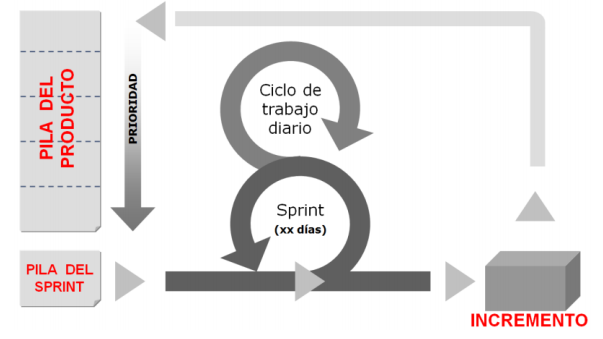
\includegraphics[width=\linewidth]{scrum.png}
  \caption{Diagrama del ciclo iterativo scrum}
  \label{fig:scrum}
\end{figure}

El marco técnico de scrum, \cite{scrum2016} está formado por un conjunto de prácticas y reglas que dan respuesta a los siguientes principios de desarrollo ágil:
\begin{itemize}
	\item Gestión evolutiva del producto, en lugar de la tradicional o predictiva.
	\item Calidad del resultado basado en el \textbf{conocimiento tácito de las personas}, antes que en el explícito de los procesos y la tecnología empleada.
	\item Estrategia de \textbf{desarrollo incremental} a través de iteraciones (sprints).
\end{itemize}

Con la visión general del proyecto, y a partir de ella se especifica y da detalle a las funcionalidades que se desean obtener en primer lugar. Cada ciclo de desarrollo o iteración (\textbf{sprint}) finaliza con la entrega de una parte operativa del producto (\textbf{incremento}). La duración de cada sprint ha sido entre una semana y dos meses.\\

Para diseñar el modelo de datos y la documentación se empleará UML (Lenguaje Unificado de Modelado) y un paradigma de programación OO (Orientado a Objetos). Además se buscará usar una arquitectura MVC (Modelo Vista Controlador) y tener cada parte lo más independiente posible del resto. Esta elección podrá permitir además una mejor integración entre todos los componentes y una mayor facilidad de mantenimiento y ampliación en el futuro.

\section{Planificación del proyecto}
En primer lugar, se realiza una planificación inicial y una investigación sobre las directrices que marca Barbara Kitchenham para crear una revisión sistemática de la literatura sobre un área determinada. Dentro de esta planificación inicial se comprueba que es necesario realizar un sistema de gestión para las distintas revisiones sistemáticas de un usuario, así como un sistema de búsquedas de referencias bibliográficas que pueda sincronizar toda la información con el gestor de referencias Mendeley, y, finalmente, su posterior clasificación según los criterios indicados por el usuario y la exportación de conclusiones finales.\\

Una vez realizada la planificación inicial y analizado todos los objetivos principales del proyecto se decide realizar el desarrollo del proyecto en dos subproyectos. El primero de ellos, será la aplicación web, donde el usuario podrá acceder a todas las opciones para las creaciones de las revisiones sistemáticas de la literatura. Por otro lado, el segundo de ellos consistirá en la creación de una librería JAR donde incluirá todo el proceso de búsquedas de referencias bibliográficas en segundo plano y de manera paralela a cualquier otra búsqueda que se realice. Esta librería, deberá ser incluida en el primer subproyecto, por lo que necesitará de un periodo de tiempo para integrar ambas aplicaciones.\\

Con toda esta información, se opta por dividir el roceso en ocho hitos tal y como podemos ver en la tabla \ref{table:hitos}. El tiempo se indica en dias. Cada uno de estos hitos, tendrá asociados varias subtareas o subobjetivos que deberán realizarse para dar por bueno el hito principal. El hito 0 corresponderá a la adquisición de conocimientos mientras que el hito 7 es asignado a la redacción de la memoria.\\

\begin{table}[!hbt]
	\begin{center}
		\begin{tabular}{|p{2cm}|p{6cm}|p{2.5cm}|p{2.5cm}|}
			\hline
			\textbf{Sprint} & \textbf{Descripción} & \textbf{Estimado} & \textbf{Real}\\
			\hline
			Hito 0 & Propuesta inicial del proyecto & 7 & 5\\
			\hline
			Hito 1 & Investigación y adquisición de conocimientos & 50 & 63\\
			\hline
			Hito 2 & Desarrollo Aplicación Web & 110 & 160\\
			\hline
			Hito 3 & Desarrollo Aplicación Mendeley-REST en Java & 60 & 100\\
			\hline
			Hito 4 & Integración de aplicaciones & 30 & 26\\
			\hline
			Hito 5 & Pruebas del sistema y rendimiento & 10 & 5\\
			\hline
			Hito 6 & Despliegue de la aplicación & 20 & 25\\
			\hline
			Hito 7 & Redacción de memoria & 180 & 280\\
			\hline
		\end{tabular}
		\caption{Tiempo estimado frente a tiempo real de cada Sprint}
		\label{table:hitos}
	\end{center}
\end{table}

Para mostrar el desarrollo detallado de toda la aplicación y desarrollo del software se muestran en las figuras \ref{fig:gantt01}, \ref{fig:gantt02}, \ref{fig:gantt03}, \ref{fig:gantt04} y \ref{fig:gantt05} unos diagramas de Gantt ordenados cronológicamente haciendo referencia a cada uno de los hitos que hemos explicado anteriormente. Los diagramas han sido realizados con la herramienta GanttProject \cite{gantt15}. Cabe indicar, que el hito de mayor duración es el último, que corresponde a la redacción de la documentación de este proyecto, ya que se ha ido redactando a medida que se ha ido completando cada una de las fases del proyecto.\\

\begin{figure}[h!]
	\begin{center}
		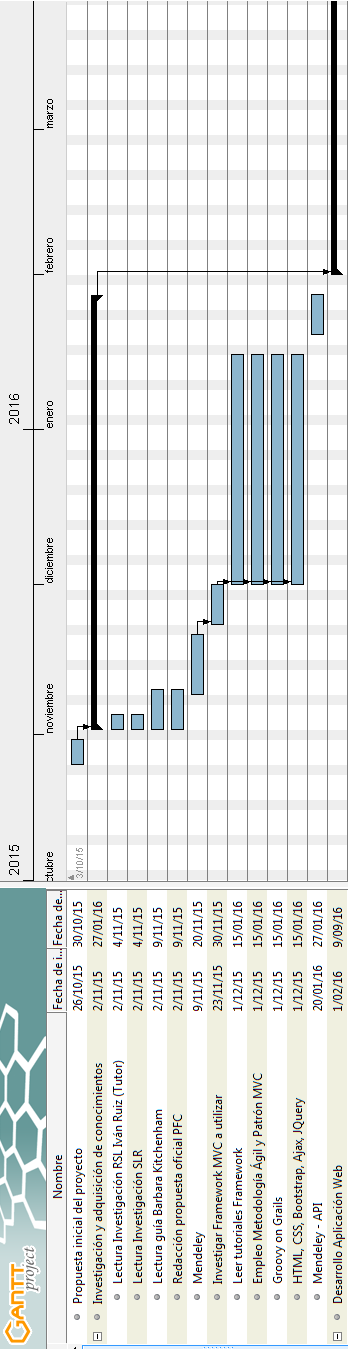
\includegraphics[width=10cm, height=20cm]{gant01.png}
		\caption{Diagrama de Gantt con la propuesta inicial y la adquisición de conocimientos.}
		\label{fig:gantt01}
	\end{center}
\end{figure}

\begin{figure}[h!]
	\begin{center}
		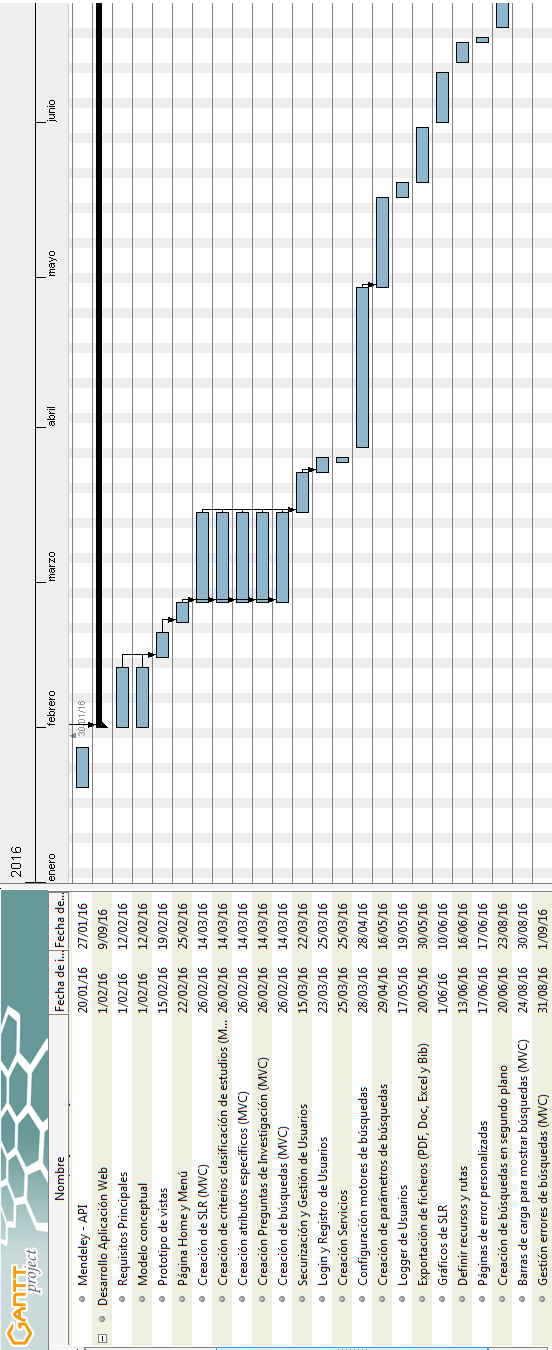
\includegraphics[width=10cm, height=20cm]{gant02.png}
		\caption{Diagrama de Gantt con el Desarrollo de la Aplicación Web.}
		\label{fig:gantt02}
	\end{center}
\end{figure}

\begin{figure}[h!]
	\begin{center}
		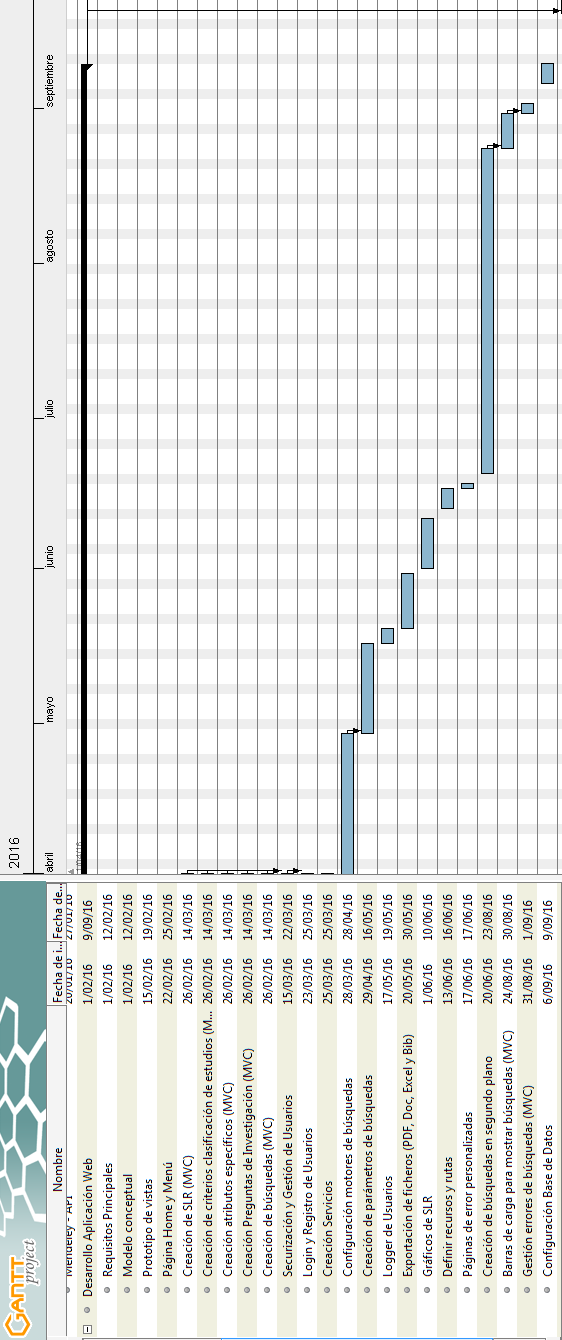
\includegraphics[width=10cm, height=20cm]{gant03.png}
		\caption{Diagrama de Gantt con el Desarrollo de la Aplicación Web (II).}
		\label{fig:gantt03}
	\end{center}
\end{figure}

\begin{figure}[h!]
	\begin{center}
		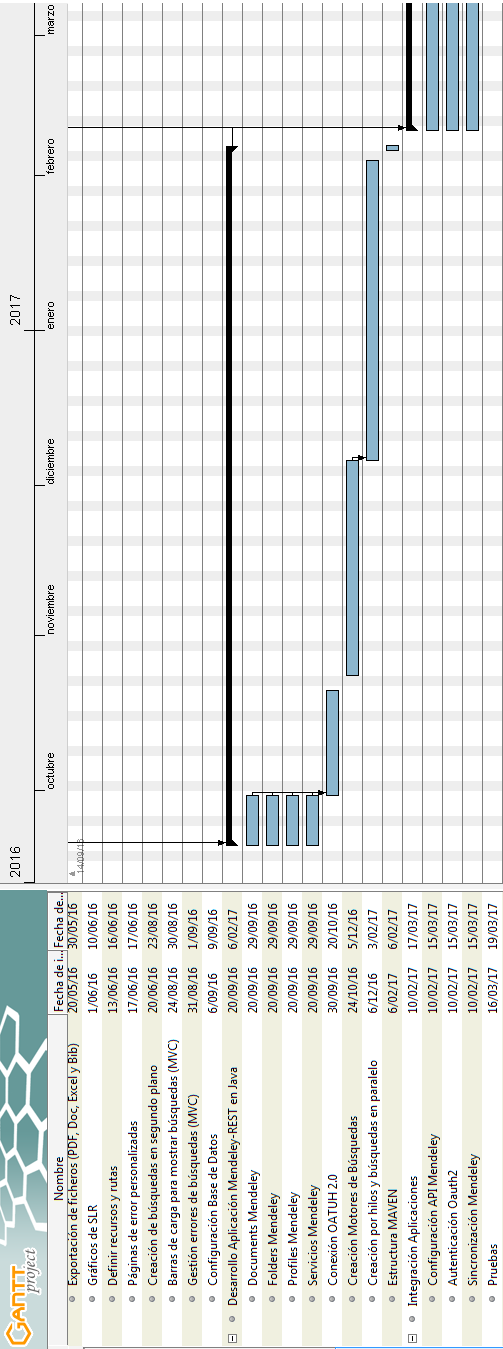
\includegraphics[width=10cm, height=20cm]{gant04.png}
		\caption{Diagrama de Gantt con el Desarroll de la Aplicación Mendeley-REST en Java.}
		\label{fig:gantt04}
	\end{center}
\end{figure}

\begin{figure}[h!]
	\begin{center}
		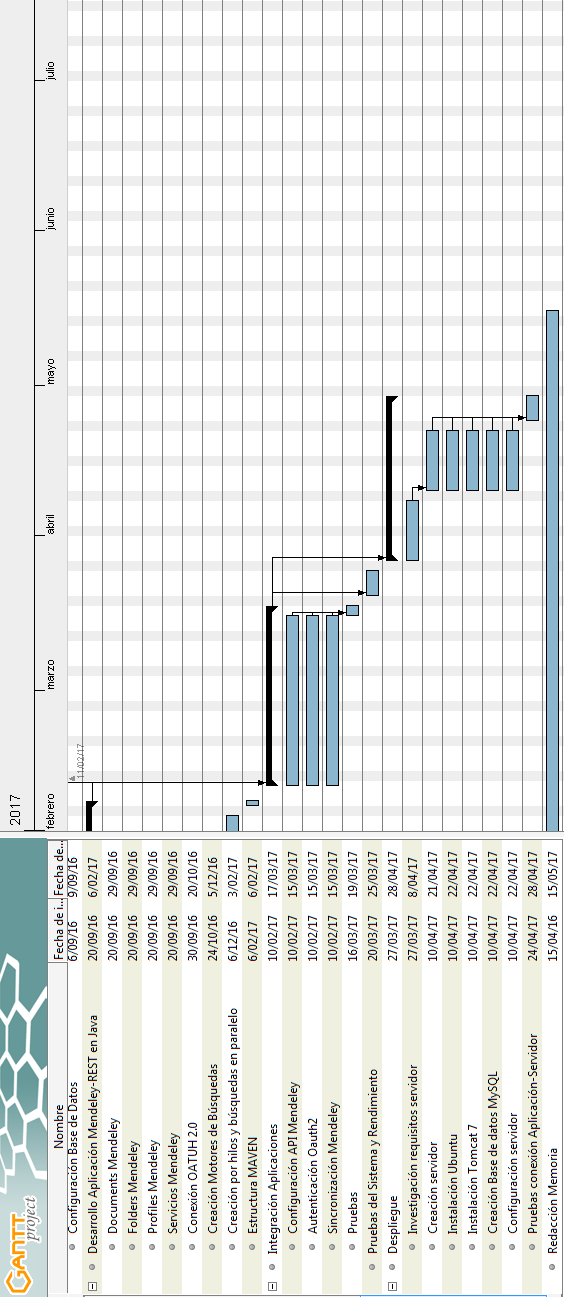
\includegraphics[width=10cm, height=20cm]{gant05.png}
		\caption{Diagrama de Gantt con la Integración de Aplicaciones, Despliegue y Redacción de la memoria.}
		\label{fig:gantt05}
	\end{center}
\end{figure}

%Estimación temporal y definición del calendario básico (hitos principales e iteraciones). Desarrollo de la planificación detallada, utilizando un diagrama de Gantt. Los diagramas de Gantt que se vean correctamente (girados y divididos si hace falta).\\

%Se debe incluir una comparación cuantitativa del tiempo y el esfuerzo realmente invertido frente al estimado y planificado. Estos datos pueden recogerse del sistema de gestión de tareas empleado para el seguimiento del proyecto.



\section{Organización}
En este apartado recogemos las personas o roles que se encuentran involucrados en el proyecto así como una relación de los recursos inventariables utilizados en el proyecto: equipamiento informático, herramientas empleadas, etc.

\subsection{Roles}
En los proyectos que siguen una metodología ágil por SCRUM podemos encontrarnos con tres tipos de roles \cite{scrum2016}:

\begin{itemize}
	\item \textbf{Dueño del producto.} Es el representante del cliente, el cuál conoce el entorno de negocio del cliente, las necesidades y el objetivo que se persigue con el sistema que se construye. Tiene la visión del producto, así como las necesidades concretas del proyecto, para poder priorizar eficientemente el trabajo. El tutor de este proyecto es el más claro ejemplo de representante, así como la UCA ejerce de cliente.
	\item \textbf{Equipo de desarrollo.} Grupo o grupos de trabajo que desarrollan el producto. Todos conocen y comprenden la visión del proprietario del producto. Además, aportan y colaboran con el proprietario en el desarrolo de la pila del producto. En este proyecto el equipo está compuesto únicamente por el autor.
	\item \textbf{Scrum master.} Es el responsable del cumplimiento de las reglas de un marco de scrum técnico, asegurando que se entienden en la organización, y se trabaja confirme a ellas. Además, proporciona la asesoría y formación necesaria al proprietario del producto y al equipo. En el proyecto estará representado por el autor, por lo que éste representará tanto al equipo de desarrollo como al scrum master.
\end{itemize}

\subsection{Recursos}
En este apartado se van a listar todos los recursos inventariables de hardware y software, así como las herramientas utilizadas y los lenguajes de programación.\\

En primer lugar se listan los recursos de hardware.\\

\begin{itemize}
	\item Equipo donde se ha realizado el proyecto: Toshiba Satellite L750/L755, Intel  \textregistered Core \texttrademark  i5-2410M CPU @ 2.30GHz x 2, 4GB RAM
	\item Servidor donde se ha desplegado el proyecto: 1 vCore CPU, 2048MB RAM, 40 GB SSD Storage, 2000 GB Bandwitch
\end{itemize}

A continuación se listan los recursos de software
\begin{itemize}
	\item Equipo donde se ha realizado el proyecto:
	
	\begin{itemize}
		\item SO: Windows 7 64 bits
		\item API Externa: Google Charts y Mendeley
	\end{itemize}
	
	\item Servidor donde se ha desplegado el proyecto:
	
	\begin{itemize}
		\item SO: Ubuntu 16.04 7 64 bits
		\item Contenedor Web: Tomcat 7 64 bits
		\item Base de Datos: MySql
	\end{itemize}
\end{itemize}

A continuación se listan las herramientas empleadas.\\
\begin{itemize}
	\item IDE: Grails Tool Suite
	\item Control de versiones: Subversion
	\item Forja: Assembla
	\item SGBD: Mysql
	\item Diseño de diagramas: DIA
	\item Diseño de Mockups: Balsamiq Mockups
	\item Navegadores empleados: Firefox y Google Chrome
	\item Memoria y presentación: \LaTeX
	\item Procesador de texto: Microsoft Word 2010
	\item Gestión Hojas de cálculo: Microsoft Excel 2010
	\item Vision de documentos: Adobe Acrobat Reader
\end{itemize}

Para finalizar, se listan los lenguajes de programación utilizados:\\
\begin{itemize}
	\item Groovy
	\item Java
	\item JavaScript
	\item Ajax
	\item JQuery
	\item CSS3
	\item Bootstrap
	\item HTML
\end{itemize}

\section{Costes}
Para poder realizar una estimación de los costes del proyecto debemos tener en cuenta tanto los recursos humanos como los recursos en material empleados. Los costes indirectos como papel, bolígrafo, electricidad o conexión a Internet son los que denominaremos ``Costes indirectos``. El porcentaje de su valor puede oscilar entre el 10\% y el 20\% del gasto del personal, tomaremos el gasto medio de dicho intervalo, es decir, un 15\%.\\

De los recursos hardware debemos tener en cuenta tanto el equipo empleado para el desarrollo. Normalmente, los ordenadores suelen tener un periodo de amortización entre los 2 y 4 años. Al igual que antes, tomaremos la media de este periodo, 3 años. Si el equipo costó 750 euros, se amortizan unos 250 euros al año y como el tiempo de desarrollo del proyecto es de entre 2 y 3 años a tiempo parcial, tomaremos 2,5 años como periodo medio y el coste final será de 625 euros. El coste del servidor son de unos 10 euros al mes, sólamente ha estado desplegado en el servidor alrededor de 3 meses, por lo que su gasto alcanza los 30 euros.\\

Con respecto a los recursos del software, no tendrá ningún gasto, puesto que el sistema operativo Windows 7 viene incluido en los gastos del equipo con el que se ha desarrollado el proyecto, así como los paquetes informáticos (hojas de cálculo y editor de texto). Además, el servidor tiene instalado Ubuntu y tampoco supone ningún gasto económico puesto que viene en el gasto mensual del servidor.\\

Para el cálculo de costes de personal se ha consultado las tablas salariales de la UCA para el personal técnico de apoyo contratado laboral \cite{paslaboral}. El coste es de unos 20.298,30 euros anuales, lo equivale a 1.353,22 euros mensuales. Como el tiempo dedicado en este tiempo ha sido lo correspondiente a media jornada, tomaremos como un gasto mensual de 676.61 euros. De esta manera, el coste anual será de unos 8119.32 euros y alcanzaremos unos gastos anuales de 20298 euros.\\

En la tabla \ref{table:costes} desglosamos los costes mensuales y totales del proyecto:

\begin{table}[!hbt]
	\begin{center}
		\begin{tabular}{|p{2cm}|p{6cm}|p{2.5cm}|p{2.5cm}|}
			\hline
			\textbf{Unidades} & \textbf{Descripción} & \textbf{Coste Unitario} & \textbf{Coste total}\\
			\hline
			1 & Ingeniero Técnico Informático & 8119.32 \euro/año & 20298 \euro\\
			\hline
			1 & Ordenador personal & 286.67 \euro/año & 625 \euro\\
			\hline
			1 & Alquiler Host & 10 \euro/mes & 30 \euro\\
			\hline
			1 & Costes indirectos & 1217 \euro/año & 3044 \euro\\
			\hline
			\multicolumn{3}{|c|}{\textbf{Total}} & 23967 \euro\\
			\hline
		\end{tabular}
		\caption{Costes del desarrollo}
		\label{table:costes}
	\end{center}
\end{table}

%Estudio y presupuesto de los costes de los recursos (humanos y materiales) descritos anteriormente, necesarios para el proyecto.

%Para el cálculo de costes de personal pueden consultarse las tablas salariales de la UCA para el personal técnico de apoyo contratado laboral \cite{paslaboral}, o bien otras más ajustadas a la realidad. El cálculo del coste del personal del proyecto debe hacerse en personas-mes, y luego hacer la correspondencia al coste monetario.\\

\section{Riesgos}
En esta sección vamos a describir los posibles riesgos del proyecto ordenados de mayor a menor prioridad, indicando su posible impacto (efecto que la ocurrencia del citado riesgo tendría en el desarrollo del proyecto) y la probabilidad de ocurrencia. Además, indicamos el plan necesario para reducir los efectos del riesgo una vez se haya materializado o disminuir que este ocurra. Esta información viene recogida en la tabla \ref{table:riesgos}.

\begin{table}[!hbt]
	\begin{center}
		\begin{tabular}{|p{3.5cm}|p{1.5cm}|p{2cm}|p{6cm}|}
			\hline
			\textbf{Riesgo} & \textbf{Prob.} & \textbf{Magnitud} & \textbf{Plan a realizar}\\
			\hline
			Tiempo infraestimado para el desarrollo de las tareas & 30\% & 5-8 semanas & Se comunica al tutor del proyecto del posible retraso, modificando la planificación temporal del proyecto o bien el plazo de entrega para poder finalizarlo.\\
			\hline
			Desarrollo de métodos y funciones software incorrectos & 30\% & 3-4 semanas & Se comprueba la calidad del código y su validez, para así evitar el denominado \textbf{DRY} (\textit{Don't Repeat yourself}) y estudiar su re-utilización una vez corregido.\\
			\hline
			Cambios en API de Mendeley & 30\% & 3 semanas & Comunicar al tutor del proyecto del posible retraso y realizar una rápida investigación de los cambios producidos en la API de Mendeley, así como el desarrollo de la nueva implementación de la misma.\\
			\hline
			Cambios en API de motores de búsquedas de referencias bibliográficas & 30\% & 3 semanas & Comunicar al tutor del proyecto del posible retraso y realizar una rápida investigación de los cambios producidos en los motores de búsquedas, como el desarrollo de la nueva implementación de los mismos.\\
			\hline
			Elección incorrecta en las herramientas empleadas de desarrollo & 15\% & 2-3 semanas & Comunicar al tutor del proyecto del posible retraso y realizar una rápida investigación de las nuevas herramientas a emplear, así como de la búsqueda y lectura de documentación.\\
			\hline
			Paro del proyecto & 20\% & 1-2 semanas & Revisar la planificación y ajustarla, así como añadir horas extras una vez que se retome el desarrollo.\\
			\hline
			Problemas en los tests & 30\% & 1-2 semanas & Se analizan los tests y se planteará la nueva revisión de éstos y, en el caso correspondiente, crear unos nuevos.\\
			\hline
		\end{tabular}
		\caption{Lista de riesgos del proyecto}
		\label{table:riesgos}
	\end{center}
\end{table}

%Enumeración de los riesgos del proyecto, indicando su posible impacto (efecto que la ocurrencia del citado riesgo tendría en el desarrollo del proyecto) y la probabilidad de ocurrencia. Una vez los riesgos son identificados y priorizados, hay que definir los planes necesarios para reducir los efectos del riesgo una vez se haya materializado o disminuir que este ocurra.\\

\section{Aseguramiento de calidad}
Para asegurar el cumplimiento de la calidad de este se contempla los siguientes aspectos:\\

\begin{itemize}
	\item Realización de controles o pruebas para asegurar su calidad.
	\item Tomar medidas de actuación relacionadas con el control de calidad.
\end{itemize}

Se realizará un análisis para cada uno de los hitos o tareas, con lo que es necesario un plan de verificación y validación dentro de los mismos para poder asegurar la calidad del producto y el correcto funcionamiento de los mismos. Estas comprobaciones se realizarán a lo largo del proyecto y así comprobar que todo está correcto y se cumple los requisitos establecidos.\\

%En esta sección se incluirán las actividades y tareas relacionadas con el aseguramiento de calidad a realizar durante el desarrollo del software. Se incluirán los estándares, prácticas y normas aplicables durante el desarrollo del software.\\

%También, deberán recogerse los diferentes tipos de revisiones, verificaciones y validaciones que se van a llevar a cabo, los criterios para la aceptación o rechazo de cada producto y los procedimientos para implementar acciones correctoras o preventivas.
